\documentclass[10pt]{book}
\usepackage{gvv-book}
\usepackage{gvv}
\usepackage[sectionbib,authoryear]{natbib}% for name-date citation comment the below line
\usepackage{setspace}
\setstretch{1.0}
\setcounter{secnumdepth}{3}
\setcounter{tocdepth}{2}
\makeindex
\let\cleardoublepage\clearpage 
\begin{document}
\frontmatter 
%%%%%%%%%%%%%%%%%%%%%%%%%%%%%%%%%%%%%%%%%%%%%%%%%%%%%%%%%%%%%%%% 
\booktitle{Geometry}
\subtitle{Through Algebra} 
\AuAff{Errala Paulsonashish}
%\halftitlepage
\titlepage
\tableofcontents 
%\listoffigures %optional
%\listoftables  %optional   
%% before \tableofcontents
%%%%%%%%%%%%%%%%%%%%%%%%%%%%%%%%%%%%%%%%%%%%%%%%%%%%%%%%%%%%%%%%
\setcounter{page}{0} 
\begin{introduction}                                 
This book shows how to solve problems in geometry using trigonometry and coordinate geometry. 
\end{introduction}
\mainmatter
\chapter{Triangle}
Consider a triangle with vertices
                \begin{align}
                        \label{eq:tri-pts}
                        \vec{A} = \myvec{-5 \\ -4},\,
                        \vec{B} = \myvec{3 \\ -3},\,
                        \vec{C} = \myvec{4 \\ 0}  
		\end{align} 
\section{Median}
\begin{enumerate}[label=\thesection.\arabic*.,ref=\thesection.\theenumi]
\numberwithin{equation}{enumi}
\item If $\vec{D}$ divides $\vec{BC}$ in the ratio $k\colon1$,
    \begin{align}
	\vec{D}= \frac{k\vec{C}+\vec{B}}{k+1}
    \end{align}
    Find the mid points $\vec{D}, \vec{E}, \vec{F}$ of the sides $\vec{BC}, \vec{CA}$ and $\vec{AB}$ respectively.\
\solution \\
Since $\vec{D}$ is the midpoint of $\vec{BC}$,
\begin{align}
k &= 1,\\
\implies \vec{D} &= \frac{\vec{C} + \vec{B}}{2}
= \frac{1}{2}\myvec{7\\-3}
	\label{eq:median-d}
\end{align}
Similarly, $\vec{E}$ is the midpoint of $\vec{AC}$, and $\vec{F}$ is the midpoint of $\vec{AB}$,
\begin{align}
	\label{eq:median-e}
\vec{E} &= \frac{\vec{A} + \vec{C}}{2}
= \frac{1}{2}\myvec{-1\\-4}\\
\vec{F} &= \frac{\vec{A} + \vec{B}}{2}
= \frac{1}{2}\myvec{-2\\-7}
	\label{eq:median-f}
\end{align}
\begin{figure}[H]
\centering
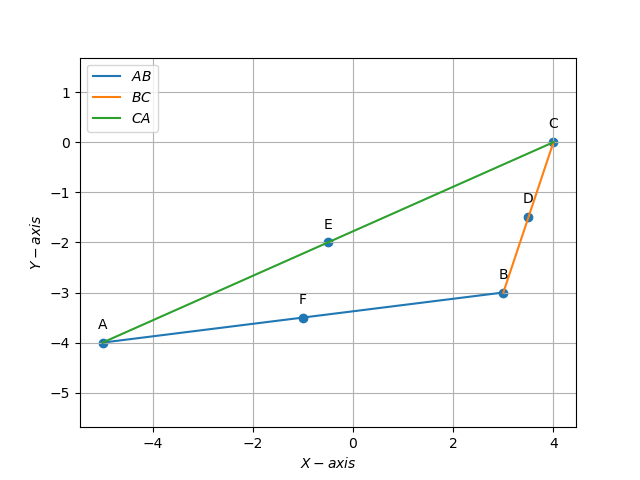
\includegraphics[width=\columnwidth]{figs/DEF_midpoints.png}
\caption{Triangle $\vec{ABC}$ with midpoints $\vec{D},\vec{E}$ and $\vec{F}$}
\label{fig:DEF_midpoints}
\end{figure}

%%1.1.2
\item Find the equations of $\vec{AD}, \vec{BE}$ and $\vec{CF}$.\\
 \solution:\\
$\vec{D}, \vec{E}$ and $\vec{F}$ are the midpoints of $\vec{BC}, \vec{CA}$ and $\vec{AB}$ respectively, then\\
\begin{align}
 \vec{D} &=  \myvec{\frac{7}{2} \\ \frac{-3}{2}}\\
 \vec{E} &=  \myvec{\frac{-1}{2} \\ -2}\\
 \vec{F} &= \myvec{-1 \\ \frac{-7}{2}}
\end{align}
\begin{enumerate}

 \item The normal equation for the median $\vec{AD}$ is
  \begin{align}
    \vec{n}^{\top}\myvec{\vec{x}-\vec{A}}&=0\\
    \implies
    \vec{n}^{\top}\vec{x}&=\vec{n}^{\top}\vec{A}
  \end{align}
 We have to find the $\vec{n}$ so that we can find $\vec{n}^{\top}$.
 Since,
\begin{align}
  \vec{n} &= \myvec{0 & 1\\
  -1 & 0}\vec{m}
\end{align}
Here $\vec{m} = \vec{D}- \vec{A}$ for median $\vec{AD}$
\begin{align}
\vec{m}&=\myvec{\frac{7}{2}\\ \frac{-3}{2}} - \myvec{-5 \\  -4}\\
       &=\myvec{\frac{17}{2}\\ \frac{5}{2}}
\end{align}
Since,
\begin{align}
  \vec{n} &= \myvec{0 & 1 \\ -1 & 0}\vec{m} \\
\implies
\vec{n} &= \myvec{0 & 1 \\ -1 & 0} \myvec{\frac{17}{2}\\ \frac{5}{2}}\\
        &= \myvec{\frac{5}{2} \\ \frac{-17}{2}} \\
        \vec{n}^{\top} = & \myvec{\frac{5}{2} & \frac{-17}{2}}
\end{align}
Hence the normal equation of median $\vec{AD}$ is 
\begin{align}
    \myvec{\frac{5}{2} & \frac{-17}{2}}\vec{x}&= \myvec{\frac{5}{2} & \frac{-17}{2}}\myvec{-5\\-4}\\
    \implies
     \myvec{\frac{5}{2} & \frac{-17}{2}}\vec{x}&= \frac{43}{2}
\end{align}

\item The normal equation for the median $\vec{BE}$ is
\begin{align}
\vec{n}^{\top}\myvec{\vec{x}-\vec{B}}&=0\\
\implies
\vec{n}^{\top}\vec{x}&=\vec{n}^{\top}\vec{B}
\end{align}
Here $\vec{m} = \vec{E}- \vec{B}$ for median $\vec{BE}$
\begin{align}
\vec{m}&=\myvec{\frac{-1}{2}\\ -2} - \myvec{3\\-3}\\
       &=\myvec{\frac{-7}{2}\\1}
\end{align}
Since,
\begin{align}
  \vec{n} &= \myvec{0 & 1\\
  -1 & 0}\vec{m}\\
\implies
\vec{n} &= \myvec{0 & 1\\
  -1 & 0}\myvec{\frac{-7}{2}\\1}\\
        &= \myvec{1\\ \frac{7}{2}}\\
        \vec{n}^{\top} = &\myvec{1 & \frac{7}{2}}
\end{align}
Hence, the normal equation of median $\vec{BE}$ is 
\begin{align}
    \myvec{1 & \frac{7}{2}}\vec{x}&=\myvec{1 & \frac{7}{2}}\myvec{3\\-3}\\
\implies
    \myvec{1 & \frac{7}{2}}\vec{x}&=\frac{-15}{2}
\end{align}

\item The normal equation for the median $\vec{CF}$ is
\begin{align}
\vec{n}^{\top}\myvec{\vec{x}-\vec{C}}&=0\\
\implies
\vec{n}^{\top}\vec{x}&=\vec{n}^{\top}\vec{C}
\end{align}
Here $\vec{m} = \vec{F}- \vec{C}$ for median $\vec{CF}$
\begin{align}
\vec{m}&=\myvec{-1 \\ \frac{-7}{2}} - \myvec{4\\0}\\
       &=\myvec{-5 \\ \frac{-7}{2}}
\end{align}
Since,
\begin{align}
  \vec{n} &= \myvec{0 & 1\\
  -1 & 0}\vec{m}\\
\implies
\vec{n} &= \myvec{0 & 1\\
  -1 & 0}\myvec{-5 \\ \frac{-7}{2} }\\
        &= \myvec{\frac{-7}{2} \\ -5} \\
        \vec{n}^{\top} = &\myvec{\frac{-7}{2} & 5}
\end{align}
Hence the normal equation of median $\vec{CF}$ is 
\begin{align}
    \myvec{\frac{-7}{2} & 5 }\vec{x}&=\myvec{\frac{-7}{2} & 5}\myvec{4\\0}\\
    \implies
    \myvec{\frac{-7}{2} & 5}\vec{x}&=-14
\end{align}
\end{enumerate}
\begin{figure}[H]
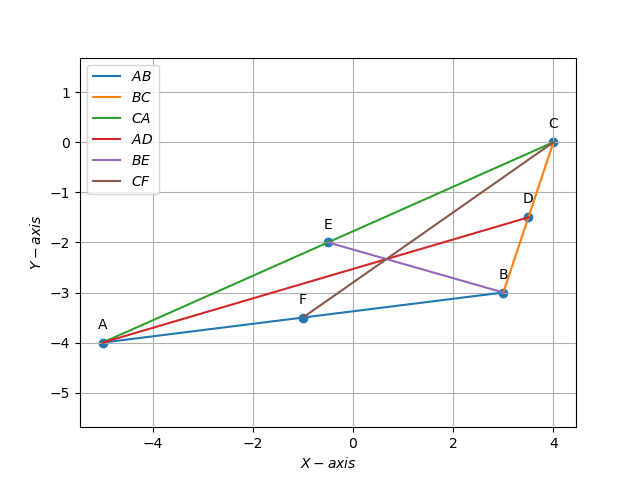
\includegraphics[width=\columnwidth]{figs/DEF_medians.png}
\caption{ Medians $AD$ , $BE$ and $CF$}
\label{fig:DEF_medians}
\end{figure}

%Question 1.2.3:
\item Find the intersection $\vec{G}$ of $\vec{BE}$ and $\vec{CF}$
\\ 
\solution \\
$\vec{A},\vec{B}$ and $\vec{C}$ are vertices of triangle:
\begin{align}
    \vec{A} &= \myvec{-5 \\-4} \\
    \vec{B} &= \myvec{3 \\ -3} \\
    \vec{C} &= \myvec{4 \\ 0}
\end{align}
Since $\vec{E}$ and $\vec{F}$ are midpoints of $\vec{CA}$ and $\vec{AB}$,
\begin{align}
    \vec{E} &= \frac{\vec{A} + \vec{C}}{2} \\
	&= \myvec{\frac{-1}{2} \\-2}\\
    \vec{F} &= \frac{\vec{B} + \vec{A}}{2} \\ 
    &= \myvec{ -1 \\ \frac{-7}{2}}
\end{align}
The line $\vec{BE}$ in vector form is given by
\begin{align}
\myvec{1 & \frac{7}{2}} \vec{x} &= \frac{-15}{2}
\label{eq:1.2.3,8}
\end{align}
The line $\vec{CF}$ in vector form is given by
\begin{align}
\myvec{ \frac{-7}{2}& 5} \vec{x} &= -14
\label{eq:1.2.3,9}
\end{align}
From \eqref{eq:1.2.3,8} and \eqref{eq:1.2.3,9} the augmented matrix is:
\begin{align}
\myvec{
1 & \frac{7}{2} & \frac{-15}{2} \\
\frac{-7}{2} & 5 & -14
}
\end{align}
Solve for $\vec{G}$ using Gauss-Elimination method :
\begin{align}
    \label{eq:matrowoperations}
 \myvec{
1 & \frac{7}{2} & \frac{-15}{2} \\
\frac{-7}{2} & 5 & -14
}
\xleftrightarrow[]{R_2 \leftarrow R_2+\frac{7R_1}{2}}
    \myvec{
    1 & \frac{7}{2} & \frac{-15}{2}
    \\
    0 & \frac{69}{4} & \frac{-161}{4} 
    }
    \\
     \xleftrightarrow[]{R_2\leftarrow \frac{4R_2}{69}}
    \myvec{
    1 & \frac{7}{2} & \frac{-15}{2}
    \\
    0 & 1 & \frac{-7}{3} 
    }
    \\
     \xleftrightarrow[]{R_1\leftarrow R_1-\frac{7R_2}{2}}
    \myvec{
    1 & 0 & \frac{2}{3}
    \\
    0 & 1 & \frac{-7}{3}
    }
\end{align} 
Therefore, 
\begin{align}
\vec{G} = \myvec{\frac{2}{3} \\ \frac{-7}{3}}
\end{align}
From  \figref{fig:G_centroid}, We can see that $\vec{G}=\myvec{\frac{2}{3}\\ 
\frac{-7}{3}}$ is the intersection of $\vec{BE}$ and $\vec{CF}$.
\begin{figure}[H]
\centering
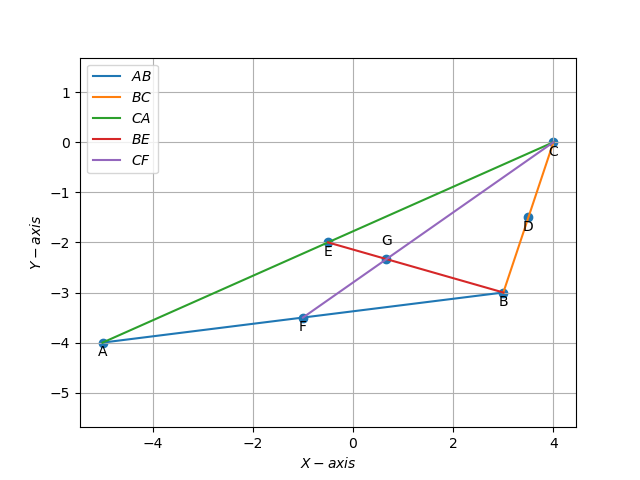
\includegraphics[width=\columnwidth]{figs/G_centroid.png}
\caption{$G$ is the centroid of triangle $ABC$}
\label{fig:G_centroid}
\end{figure}

%Question 1.2.4:
\item Verify that 
		\begin{align}
			\frac{BG}{GE} = 
			\frac{CG}{GF} =
			\frac{AG}{GD} =2 
		\end{align}\\

\solution \\
In order to verify the above equation we first need to find $\vec{G}$.\\
$\vec{G}$ is the intersection of $\vec{BE}$ and $\vec{CF}$, Using the value of $\vec{G}$ from (1.2.3).
\begin{align}
		\vec{G} = \myvec{\frac{2}{3} \\ \frac{-7}{3}}
\end{align}
Also, We know that $\vec{D}, \vec{E}$ and $\vec{F}$ are midpoints of $\vec{BC}, \vec{CA}$ and $\vec{AB}$ respectively from (1.2.1).
\begin{align}
		\vec{D} = \myvec{\frac{7}{2} \\ \frac{-3}{2}},\,
		\vec{E} = \myvec{\frac{-1}{2} \\ -2},\,
		\vec{F} = \myvec{-1 \\ \frac{-7}{2}}
\end{align}
\begin{enumerate}
\item Calculating the ratio of $\vec{BG}$ and $\vec{GE}$ ,
\begin{align}
		\label{eq:tri-pts/4} \vec{G}-\vec{B} &= \myvec{\frac{-7}{3} \\ \frac{2}{3}} \\
		\label{eq:tri-pts/5} \vec{E}-\vec{G} &= \myvec{\frac{7}{6} \\ \frac{1}{3}} \\
		\label{eq:tri-pts/6} \norm{\vec{G}-\vec{B}} &= \sqrt{\brak{\frac{7}{3}}^2 + \brak{\frac{2}{3}}^{2}} &= \frac{\sqrt{53}}{3} \\
		\label{eq:tri-pts/7} \norm{\vec{E}-\vec{G}} &= \sqrt{\brak{\frac{7}{6}}^2 + \brak{\frac{1}{3}}^2} &= \frac{\sqrt{53}}{6} \\
		\label{eq:tri-pts/8}\frac{BG}{GE} &= \frac{\norm{\vec{G}-\vec{B}}}{\norm{\vec{E}-\vec{G}}} &= \frac{\frac{\sqrt{53}}{3}}{\frac{\sqrt{53}}{6}} &= 2  
\end{align}		
\item Calculating the ratio of $\vec{CG}$ and $\vec{GF}$ ,
\begin{align}
		\label{eq:tri-pts/9} \vec{G}-\vec{C} &= \myvec{\frac{-10}{3} \\ \frac{-7}{3}} \\
		\label{eq:tri-pts/10} \vec{F}-\vec{G} &= \myvec{\frac{-5}{3} \\ \frac{7}{6}} \\
		\label{eq:tri-pts/11} \norm{\vec{G}-\vec{C}} &= \sqrt{\brak{\frac{-10}{3}}^{2} + \brak{\frac{-7}{3}}^{2}} &= \frac{\sqrt{149}}{3} \\  
		\label{eq:tri-pts/12} \norm{\vec{F}-\vec{G}} &= \sqrt{\brak{\frac{-5}{3}}^{2} + \brak{\frac{7}{6}}^{2}} &= \frac{\sqrt{149}}{6} \\
		\label{eq:tri-pts/13}\frac{CG}{GF} &= \frac{\norm{\vec{G}-\vec{C}}}{\norm{\vec{F}-\vec{G}}} &= \frac{\frac{\sqrt{149}}{3}}{\frac{\sqrt{149}}{6}} &= 2		
\end{align}
\item Calculating the ratio of $\vec{AG}$ and $\vec{GD}$ ,
\begin{align}
		\label{eq:tri-pts/14} \vec{G}-\vec{A} &= \myvec{\frac{17}{3} \\ \frac{5}{3}} \\
		\label{eq:tri-pts/15} \vec{D}-\vec{G} &= \myvec{\frac{17}{6} \\ \frac{5}{6}} \\
		\label{eq:tri-pts/16} \norm{\vec{G}-\vec{A}} &= \sqrt{\brak{\frac{17}{3}}^{2} + \brak{\frac{5}{3}}^{2}} &= \frac{\sqrt{314}}{3} \\
		\label{eq:tri-pts/17} \norm{\vec{D}-\vec{G}} &= \sqrt{\brak{\frac{17}{6}}^{2}+\brak{\frac{5}{6}}^{2}} &= \frac{\sqrt{314}}{6} \\
		\label{eq:tri-pts/18}\frac{AG}{GD} &= \frac{\norm{\vec{G}-\vec{A}}}{\norm{\vec{D}-\vec{G}}} &= \frac{\frac{\sqrt{314}}{3}}{\frac{\sqrt{314}}{6}} &= 2 
\end{align}
\end{enumerate}

From \eqref{eq:tri-pts/8}, \eqref{eq:tri-pts/13}, \eqref{eq:tri-pts/18}
\begin{align}
		\frac{BG}{GE} = 
		\frac{CG}{GF} =
		\frac{AG}{GD} = 2
\end{align}
Hence verified.


%Question 1.2.5 :
\item Show that $\vec{A}, \vec{G}$ and $\vec{D}$ are collinear.\\
\solution 
Given that,
\begin{align}
    \vec{A} = \myvec{-5\\-4}
    \quad
    \vec{B} &= \myvec{3\\-3}
    \quad
    \vec{C} = \myvec{4\\0}
\end{align}
We need to show that points $\vec{A},\vec{D},\vec{G}$ are collinear.
From Problem 1.2.3 We know that, The point $\vec{G}$ is 
\begin{align}
    \vec{G} &=\myvec{\frac{2}{3}\\ \frac{-7}{3}}
\end{align}
And from Problem 1.2.1 We know that, The point $\vec{D}$ is 
\begin{align}
    \vec{D} &=\myvec{\frac{7}{2}\\ \frac{-3}{2}}
\end{align}
In Problem 1.1.3, There is a theorem/law mentioned i.e.,

Points $\vec{A},\vec{D},\vec{G}$ are defined to be collinear if 
\begin{align}
    \text{rank}\myvec{
    1 & 1 & 1\\
    \vec{A} & \vec{D} & \vec{G} \\
    } &= 2 
\end{align} 
Using the above law/Theorem Let
\begin{align}
    \vec{R}&=\myvec{
    1 & 1 & 1
    \\
    -5 & \frac{7}{2} & \frac{2}{3}
    \\
    -4  & \frac{-3}{2} & \frac{-7}{3}
    } 
\end{align} 
The matrix $\vec{R}$ can be row reduced as follows,
\begin{align}
    \label{eq:mat_row_operations}
    \myvec{
    1 & 1 & 1
    \\
    -5 & \frac{7}{2} & \frac{2}{3}
    \\
    -4  & \frac{-3}{2} & \frac{-7}{3}
    }
     \xleftrightarrow[]{R_2 \leftarrow R_2+5R_1}
    \myvec{
    1 & 1 & 1
    \\
    0 & \frac{17}{2} & \frac{17}{3}
    \\
    -4 & \frac{-3}{2} & \frac{-7}{3} 
    }
    \\
     \xleftrightarrow[]{R_3\leftarrow R_3+4R_1}
    \myvec{
    1 & 1 & 1
    \\
    0 & \frac{17}{2}& \frac{17}{3}
    \\
     0 & \frac{5}{2}& \frac{5}{3}
    }
    \\
     \xleftrightarrow[]{R_3\leftarrow R_3-\frac{R_2}{17}}
    \myvec{
    1 & 1 & 1
    \\
    0 & \frac{17}{2}& \frac{17}{3}
    \\
    0 & 0 & 0
    }
\end{align}
Rank of above matrix is 2.\\
Hence, we proved that that points $\vec{A},\vec{D},\vec{G}$ are collinear.

%Question 1.2.6:
\item Verify that 
		\begin{align}
			\vec{G}=\frac{\vec{A}+\vec{B}+\vec{C}}{3}
		\end{align}
$\vec{G}$ is known as the {\em centroid} of $\triangle ABC$.\\
Verify that\\
\begin{align}
 \vec{G}=\frac{\vec{A}+\vec{B}+\vec{C}}{3}   
\end{align}
\solution\\
$\vec{G}$ is known as the \underline{centroid} of $\triangle ABC$ \\
let us first evaluate the R.H.S of the equation
\begin{equation}
\begin{split}
\label{eq:centroid}
    \vec{G}&= \frac{\myvec{-5\\-4}+\myvec{3\\-3}+\myvec{4\\0}}{3}\\    
    &= \myvec{\frac{-5+3+4}{3} \\ \frac{-4-3+0}{3}}\\
     &= \myvec{\frac{2}{3}\\ \frac{-7}{3}}
\end{split}
\end{equation}
Hence verified.

%Question 1.2.7: 
\item Verify that 
		\begin{align}
\vec{A}-\vec{F}=\vec{E}-\vec{D}
		\end{align}
The quadrilateral $AFDE$ is defined to be a parallelogram.\\
Question : Verify that 
\begin{align}
	\vec{A}-\vec{F} = \vec{E}-\vec{D}
\end{align}
The quadrilateral $AFDE$ is defined to be parallelogram.\\ 
\solution \\
Given that,
\begin{align}
    \vec{A} = \myvec{-5\\-4}
    \quad
    \vec{B} &= \myvec{3\\-3}
    \quad
    \vec{C} = \myvec{4\\ 0}
\end{align}
From Problem 1.2.1 We know that, The point $\vec{D},\vec{E},\vec{F}$ is 
\begin{align}
    \vec{D} = \myvec{\frac{7}{2}\\ \frac{-3}{2} }
    \quad
    \vec{E} &= \myvec{\frac{-1}{2}\\-2}
    \quad
    \vec{F} = \myvec{-1 \\ \frac{-7}{2}}
\end{align}
Evaluating the R.H.S of the equation
\begin{align}
    \vec{A}-\vec{F}&=\myvec{-5\\-4} - \myvec{-1\\ \frac{-7}{2} }\\
    &=\myvec{ -4 \\ \frac{-1}{2} }
\end{align} 
Evaluating the L.H.S of the equation
\begin{align}
    \vec{E}-\vec{D}&=\myvec{\frac{-1}{2}\\-2}-\myvec{\frac{7}{2}\\ \frac{-3}{2} }\\
    &=\myvec{-4 \\ \frac{-1}{2} }
\end{align}	
Hence verified that, R.H.S = L.H.S i.e. ,
\begin{align}
	\vec{A}-\vec{F} = \vec{E}-\vec{D}
\end{align}

From the \figref{fig:AFDEparallelogram}, It is verified that $AFDE$ is a parallelogram\\
\begin{figure}[H]
\centering
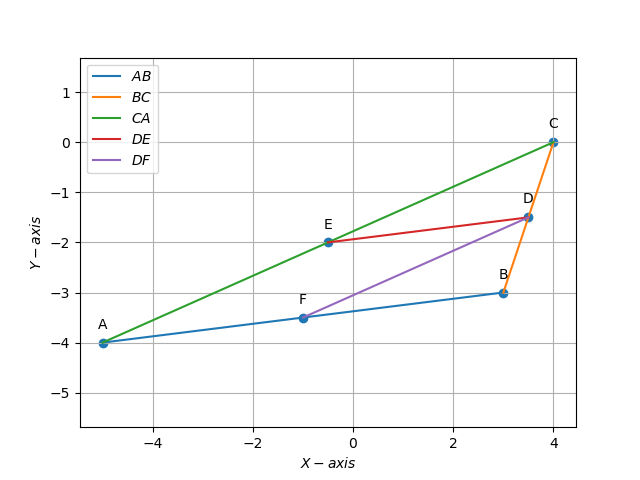
\includegraphics[width=\columnwidth]{figs/AFDE_parallelogram.png}
\caption{$AFDE$ form a parallelogram in triangle ABC}
\label{fig:AFDEparallelogram}
\end{figure}
All codes for this section are available at
\begin{lstlisting}
	geometry/Triangle/median/codes/Triangle_medians.py 
\end{lstlisting}
\end{enumerate}
\backmatter
\appendix
\latexprintindex
\end{document}
